\documentclass[12pt, twoside]{article}
\usepackage[francais]{babel}
\usepackage[T1]{fontenc}
\usepackage[latin1]{inputenc}
\usepackage[left=7mm, right=7mm, top=7mm, bottom=7mm]{geometry}
\usepackage{float}
\usepackage{graphicx}
\usepackage{array}
\usepackage{multirow}
\usepackage{amsmath,amssymb,mathrsfs}
\usepackage{soul}
\usepackage{textcomp}
\usepackage{eurosym}
 \usepackage{variations}
\usepackage{tabvar}

\pagestyle{empty}

\begin{document}

\begin{flushleft}
NOM PRENOM: \ldots \ldots \ldots \ldots \ldots \ldots \ldots \ldots \ldots
 
\bigskip

\end{flushleft}

\begin{center}
{\fbox{$5^{e}1$ \qquad \qquad \textbf{\Large{Contr�le de cours 2 (sujet 2)}}
\qquad \qquad 19/10/2009}}
\end{center}



\bigskip

\textit{Remarque: Tout le contr�le est � faire sur cette feuille. Laisser vos
traits de constructions.}


\bigskip



\begin{enumerate}
 
   \item Compl�ter:
  
     
  $6 \times 7= \ldots$ \qquad \qquad \qquad $9 \times 6 =\ldots$ \qquad \qquad
  \qquad $7 \times 7 = \ldots$ \qquad \qquad \qquad $4 \times 6 = \ldots $
  
 \bigskip 
  
  \item  Construire le sym�trique de S par rapport � T en utilisant seulement la
  r�gle.

\bigskip

 \begin{center}
 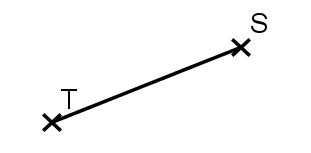
\includegraphics[width=3cm]{images/compas.png}
 
\end{center}
 
  
  \bigskip
  
  \bigskip
  
  \bigskip
 
  
  \item
   Construire le sym�trique de U par rapport � V en utilisant le compas.

 \bigskip  

 \begin{center}
 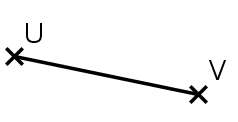
\includegraphics[width=25mm]{images/regle.png}  
\end{center}
 
  
  \bigskip
  
  
  
  \bigskip
   
   \item Compl�ter la d�finition suivante:
  
  Le sym�trique d'un point A par rapport � O est le point A' tel que \ldots
  \ldots \ldots \ldots \ldots \ldots \ldots \ldots \ldots \ldots \ldots
  
  \ldots \ldots \ldots \ldots \ldots \ldots \ldots \ldots \ldots \ldots \ldots 
  
  \bigskip
  
  
   
  \item Placer le point E tel que C et D soient sym�triques par rapport � E.
  
   \bigskip  

 \begin{center}
 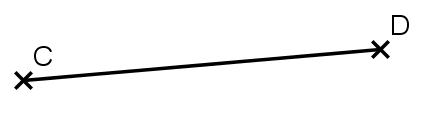
\includegraphics[width=4cm]{images/milieu.png} 
\end{center}
 
  
  \bigskip
  
  \bigskip
  
  
  \bigskip 
  
  
  \item Construire le sym�trique du segment [EF] par rapport au point G.
  
   \bigskip  

 \begin{center}
 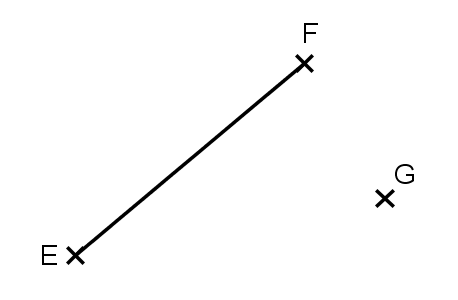
\includegraphics[width=5cm]{images/segment.png} 
\end{center}
 
  
  \bigskip  
  
  
   \bigskip  
   
    \bigskip  
 
  
  
\end{enumerate}

\end{document}
